\documentclass[a4paper,12pt]{article}
\usepackage[utf8]{inputenc}
\usepackage[MeX]{polski}
\usepackage{fixltx2e}
\usepackage[table,xcdraw]{xcolor}
\usepackage[utf8]{inputenc}
\usepackage[T1]{fontenc}
\usepackage{graphicx}
\usepackage{color}
\usepackage{mathtools}
\usepackage[font=small,labelfont=bf]{caption}
%%%%%%%%%%%%%%%%%%%%%%%%%%%%%%%%%%%%%%%%%%%%%%%%%%%%%%%%%%%%%STRONA TYTULOWA%%%%%%%%%%%%%%%%%%%%%%%%%%%%%%%%%%%%%%%%%%%%%%%%%%%%%%%%%%%%%%%%%%%%%%%%
\title{\Huge \textbf{Politechnika Wrocławska\\[0.3in]} 
  \huge Katedra Teorii Pola, Układów elektronicznych i Optoelektronicznych \\[0.2in]
  \LARGE Zespół Układów Elektronicznych
}
\date{}
\author{}

\begin{document}
\maketitle

\begin{table}[h]
  \large
  \centering
  \begin{tabular}{|ll|l|}
    \hline
    \multicolumn{1}{|l|}{Data: 7.04.2015r}                & \multicolumn{2}{l|}{Dzień: Wtorek}                                     \\ \hline
    \multicolumn{1}{|l|}{Grupa: VII}                      & \multicolumn{2}{l|}{Godzina: 12:15-15:00}                               \\ \hline
    \multicolumn{3}{|l|}{\textit{\begin{tabular}[c]{@{}l@{}}\textbf{Temat ćwiczenia:} \\ Liniowe stabilizatory napięcia\end{tabular}}} \\ \hline
    \textbf{Dane projektowe:}                             & \multicolumn{2}{l|}{}                                                 \\
    U\textsubscript{0}=11.00 V                            & \multicolumn{2}{l|}{I\textsubscript{0}=0.60 A}                         \\
    R\textsubscript{4}=0.68\Omega}                       & \multicolumn{2}{l|}{R\textsubscript{5}=3k\Omega}                          \\
    R\textsubscript{6}=1k\Omega                          & \multicolumn{2}{l|}{}\\\hline
    \multicolumn{1}{|l|}{\textbf{l.p}}                    & \textbf{Nazwisko i imię}                 & \textbf{Oceny}               \\ \hline
    \multicolumn{1}{|l|}{1}                               & Arkadiusz Ziółkowski                     &                               \\ \hline
    \multicolumn{1}{|l|}{2}                               & Jakub Koban                              &                                \\ \hline
  \end{tabular}
\end{table}
%%%%%%%%%%%%%%%%%%%%%%%%%%%%%%%%%%%%%%%%%%%%%%%%%%%%%%%%%%%%%%%%%%%%%%%%%%%%%%%%%%%%%%%%%%%%%%%%%%%%%%%%%%%%%%%%%%%%%%%%%%%%%%%%%%%%%%%%%%%%%%%%%%%%
%%%%%%%%%%%%%%%%%%%%%%%%%%%%%%%%%%%%%%%%%%%%%%%%%%%%%%%%%%%%%%%%%%%ZADANIE PROJEKTOWE%%%%%%%%%%%%%%%%%%%%%%%%%%%%%%%%%%%%%%%%%%%%%%%%%%%%%%%%%%%%%%%
%%%%%%%%%%%%%%%%%%%%%%%%%%%%%%%%%%%%%%%%%%%%%%%%%%%%%%%%%%%%%%%%%%%%%%%%%%%%%%%%%%%%%%%%%%%%%%%%%%%%%%%%%%%%%%%%%%%%%%%%%%%%%%%%%%%%%%%%%%%%%%%%%%%%
\pagebreak
\section{Zadanie projektowe}
Zaprojektować zasilacz stabilizowany o zadanych parametrach :
\begin{enumerate}
\item U\textsubscript{0}=11.00 V
\item I\textsubscript{0}=0.60 A
\end{enumerate}
%%%%%%%%%%%%%%%%%%%%%%%%%%%%%%%%%%%%%%%%%%%%%%%%%%%%%%%%%%%%%%%%%%%%%%%%%%%%%%%%%%%%%%%%%%%%%%%%%%%%%%%%%%%%%%%%%%%%%%%%%%%%%%%%%%%%%%%%%%%%%%%%%%%%
%%%%%%%%%%%%%%%%%%%%%%%%%%%%%%%%%%%%%%%%%%%%%%%%%%%%%%%%%%%%%%%%%%%CZĘŚĆ PROJEKTOWA%%%%%%%%%%%%%%%%%%%%%%%%%%%%%%%%%%%%%%%%%%%%%%%%%%%%%%%%%%%%%%%%%
%%%%%%%%%%%%%%%%%%%%%%%%%%%%%%%%%%%%%%%%%%%%%%%%%%%%%%%%%%%%%%%%%%%%%%%%%%%%%%%%%%%%%%%%%%%%%%%%%%%%%%%%%%%%%%%%%%%%%%%%%%%%%%%%%%%%%%%%%%%%%%%%%%%%
\section{Obliczenia projektowe}

\begin{equation}
  U_0=(1+\frac{R_5}{R_6})U_{REF} \quad \to \quad (1+\frac{3k\Omega}{1k\Omega})2.75 V = 11 V
\end{equation}

\begin{equation}
  R_5+R_6 \leq \frac{U_0}{1mA} \quad \to \quad 4k\Omega \leq 11k\Omega 
\end{equation}

\begin{equation}
  I_0=\frac{U_{sc}}{R_4} \quad \to \quad \frac{0.45V}{0.68\Omega}=0.66 A      
\end{equation}

%%%%%%%%%%%%%%%%%%%%%%%%%%%%%%%%%%%%%%%%%%%%%%%%%%%%%%%%%%%%%%%%%%%%%%%%%%%%%%%%%%%%%%%%%%%%%%%%%%%%%%%%%%%%%%%%%%%%%%%%%%%%%%%%%%%%%%%%%%%%%%%%%%%%
\section {Schemat projektowy}
\begin{figure}[h]
  \center
  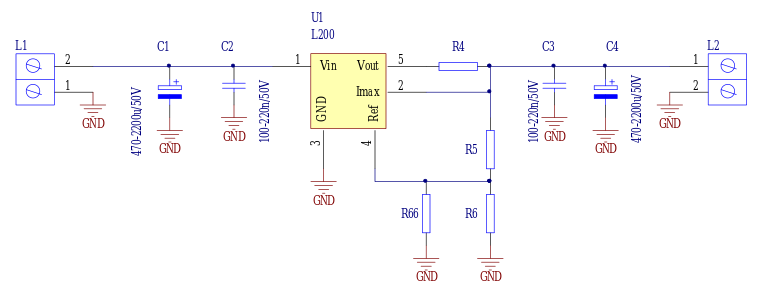
\includegraphics[width=1\textwidth]{schemat_ukladu}
  \caption{Schemat projektowanego układu}
\end{figure}
\pagebreak
%%%%%%%%%%%%%%%%%%%%%%%%%%%%%%%%%%%%%%%%%%%%%%%%%%%%%%%%%%%%%%%%%%%%%%%%%%%%%%%%%%%%%%%%%%%%%%%%%%%%%%%%%%%%%%%%%%%%%%%%%%%%%%%%%%%%%%%%%%%%%%%%%%%%
%%%%%%%%%%%%%%%%%%%%%%%%%%%%%%%%%%%%%%%%%%%%%%%%%%%%%%%%%%%%%%%%%%%CZĘŚĆ LABORATORYJNA%%%%%%%%%%%%%%%%%%%%%%%%%%%%%%%%%%%%%%%%%%%%%%%%%%%%%%%%%%%%%%
%%%%%%%%%%%%%%%%%%%%%%%%%%%%%%%%%%%%%%%%%%%%%%%%%%%%%%%%%%%%%%%%%%%%%%%%%%%%%%%%%%%%%%%%%%%%%%%%%%%%%%%%%%%%%%%%%%%%%%%%%%%%%%%%%%%%%%%%%%%%%%%%%%%%
\section{Część laboratoryjna}
\subsection{Charakterystyki napięciowe}

\begin{table}[h]
\centering
\resizebox{\textwidth}{!}{%
\begin{tabular}{|r|r|r|r|r|r|r|r|r|r|}
\hline
\multicolumn{1}{|c|}{U1{[}V{]}} & \multicolumn{2}{c|}{U2 {[}V{]}}
& \multicolumn{2}{c|}{ \partial Uwy/ \partial Uwe[\frac{V}{V}]}
& \multicolumn{1}{c|}{U1{[}V{]}} & \multicolumn{2}{c|}{U2 {[}V{]}}
& \multicolumn{2}{c|}{\partial Uwy / \partial Uwe[\frac{V}{V}]} \\ \hline
\multicolumn{1}{|l|}{}
& \multicolumn{1}{l|}{Iwy=0[A]} & \multicolumn{1}{l|}{Iwy\neq0[A]} & \multicolumn{1}{l|}{Iwy=0[A]} & \multicolumn{1}{l|}{Iwy\neq0[A]}
& \multicolumn{1}{l|}{}          & \multicolumn{1}{l|}{Iwy=0[A]} & \multicolumn{1}{l|}{Iwy\neq0[A]}
& \multicolumn{1}{l|}{Iwy=0[A]} & \multicolumn{1}{l|}{Iwy\neq0[A]} \\ \hline
0.00                        & 0.00                        & 0.00                        & \multicolumn{1}{c|}{-}      & \multicolumn{1}{c|}{-}
& 12.50                     & 10.99                       & 10.74                       & 0.00                        & 0.89\\ \hline
0.40                        & 0.00                        & 0.00                        & 0.00                        & 0.00
& 13.00                     & 10.99                       & 10.98                       & 0.00                        & 0.84\\ \hline
0.80                        & 0.00                        & 0.00                        & 0.03                        & 0.00
& 13.50                     & 10.99                       & 10.98                       & 0.00                        & 0.81\\ \hline
1.20                        & 0.01                        & 0.00                        & 0.31                        & 0.00
& 14.00                     & 11.00                       & 10.98                       & 0.00                        & 0.78\\ \hline
1.60                        & 0.14                        & 0.00                        & 0.37                        & 0.00
& 14.50                     & 11.00                       & 10.98                       & 0.00                        & 0.76\\ \hline
2.00                        & 0.29                        & 0.00                        & 0.21                        & 0.01
& 15.00                     & 11.00                       & 10.99                       & 0.00                        & 0.73\\ \hline
2.50                        & 0.39                        & 0.01                        & 4.44                        & 0.00
& 15.50                     & 11.00                       & 10.99                       & 0.00                        & 0.71\\ \hline
2.90                        & 2.17                        & 0.11                        & 0.84                        & 0.27
& 16.00                     & 11.00                       & 10.99                       & 0.00                        & 0.69\\ \hline
3.40                        & 2.59                        & 1.94                        & 0.93                        & 3.66
& 16.50                     & 11.00                       & 10.99                       & 0.00                        & 0.67\\ \hline
3.90                        & 3.03                        & 2.39                        & 0.91                        & 0.90
& 17.00                     & 11.00                       & 10.99                       & 0.00                        & 0.65\\ \hline
4.40                        & 3.49                        & 2.85                        & 1.00                        & 0.92
& 17.50                     & 11.00                       & 10.99                       & 0.00                        & 0.63\\ \hline
5.00                        & 4.09                        & 3.46                        & 0.95                        & 1.02
& 18.00                     & 11.00                       & 10.99                       & 0.00                        & 0.61\\ \hline
5.50                        & 4.56                        & 3.94                        & 0.98                        & 0.97
& 18.50                     & 11.00                       & 10.99                       & 0.00                        & 0.59\\ \hline
6.00                        & 5.05                        & 4.44                        & 0.90                        & 1.00
& 19.00                     & 11.00                       & 10.99                       & 0.00                        & 0.58\\ \hline
6.50                        & 5.50                        & 4.90                        & 0.95                        & 0.92
& 19.50                     & 11.00                       & 11.00                       & 0.00                        & 0.56\\ \hline
7.00                        & 5.95                        & 5.36                        & 1.06                        & 0.91
& 20.00                     & 11.00                       & 10.99                       & 0.00                        & 0.55\\ \hline
7.50                        & 6.48                        & 5.90                        & 1.01                        & 1.08
& 21.00                     & 11.00                       & 11.00                       & 0.00                        & 0.52\\ \hline
8.00                        & 6.99                        & 6.42                        & 0.95                        & 1.03
& 22.00                     & 11.01                       & 11.00                       & 0.00                        & 0.50\\ \hline
8.50                        & 7.46                        & 6.89                        & 0.95                        & 0.96
& 23.00                     & 11.01                       & 11.00                       & 0.00                        & 0.48\\ \hline
9.00                        & 7.87                        & 7.32                        & 1.00                        & 0.85
& 24.00                     & 11.01                       & 11.00                       & 0.00                        & 0.46\\ \hline
9.50                        & 8.37                        & 7.83                        & 0.95                        & 1.02
& 25.00                     & 11.01                       & 11.00                       & 0.00                        & 0.44\\ \hline
10.10                       & 8.92                        & 8.38                        & 1.01                        & 0.92
& 26.00                     & 11.01                       & 11.00                       & 0.00                        & 0.42\\ \hline
10.50                       & 9.32                        & 8.77                        & 1.02                        & 0.98
& 27.00                     & 11.01                       & 11.01                       & 0.00                        & 0.41\\ \hline
11.00                       & 9.87                        & 9.35                        & 0.96                        & 1.16
& 28.00                     & 11.01                       & 11.01                       & 0.00                        & 0.39\\ \hline
11.50                       & 10.35                       & 9.85                        & 0.90                        & 0.98
& 29.00                     & 11.01                       & 11.01                       & 0.00                        & 0.38\\ \hline
12.00                       & 10.78                       & 10.29                       & 0.42                        & 0.90
& 30.00                     & 11.01                       & 11.01
& \multicolumn{1}{c|}{-}    & \multicolumn{1}{c|}{-}      \\ \hline
\end{tabular}
}
\end{table}

\pagebreak
%%%%%%%%%%%%%%%%%%%%%%%%%%%%%%%%%%%%%%%%%%%%%%%%%%%%%%%%%%%%%%%%%%%%%%%%%%%%%%%%%%%%%%%%%%%%%%%%%%%%%%%%%%%%%%%%%%%%%%%%%%%%%%%%%%%%%%%%%%%%%%%%%%%%
\begin{figure}[h!]
  \center 
  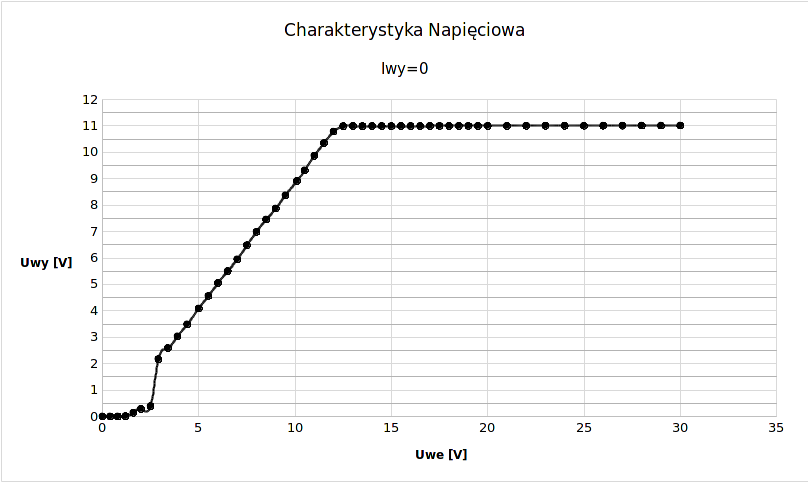
\includegraphics[width=1\textwidth]{charak-napieciowa1}
  \caption{U\textsubscript{wy}=f(U\textsubscript{we}) przu I\textsubscript{wy}=0A}
\end{figure}

\begin{figure}[h!]
  \center
  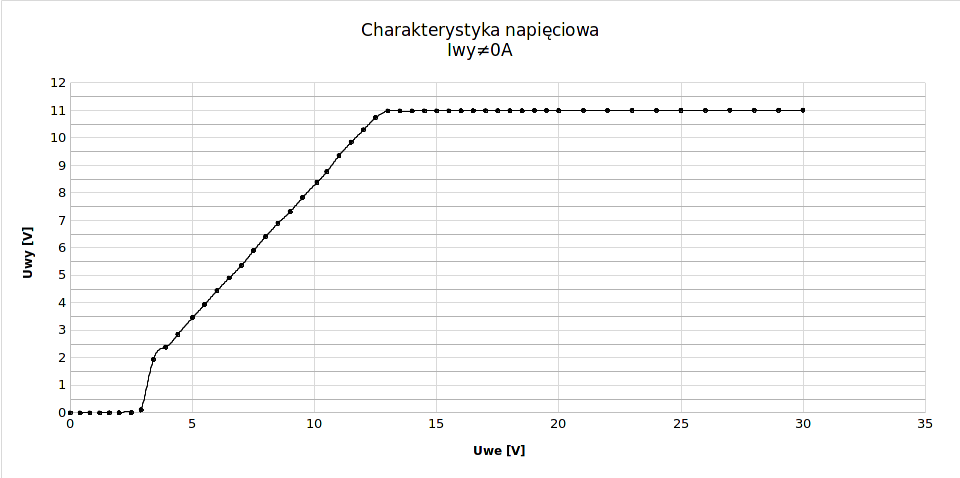
\includegraphics[width=1\textwidth]{charak-napieciowa2}
  \caption{ U\textsubscript{wy}=f(U\textsubscript{we}) przu I\textsubscript{wy}\neq0A}
\end{figure}

Analizując przedstawione charakterystyki możemy zauważyć,iż układ poprawnie stabilizuje napięcie od (odpowiednio) 12.5V i 13V aż do maksymalnego
napięcia jakie udało nam się uzyskać z zasilacza czyli 30V. Świadczy to o tym ,iż dropout jest równy odpowiednio około 1.5V i 2 V.
\pagebreak
%%%%%%%%%%%%%%%%%%%%%%%%%%%%%%%%%%%%%%%%%%%%%%%%%%%%%%%%%%%%%%%%%%%%%%%%%%%%%%%%%%%%%%%%%%%%%%%%%%%%%%%%%%%%%%%%%%%%%%%%%%%%%%%%%%%%%%%%%%%%%%%%%%%%
\subsection{Współczynnik stabilizacji napięciowej}
\begin{figure}[h!]
  \center 
  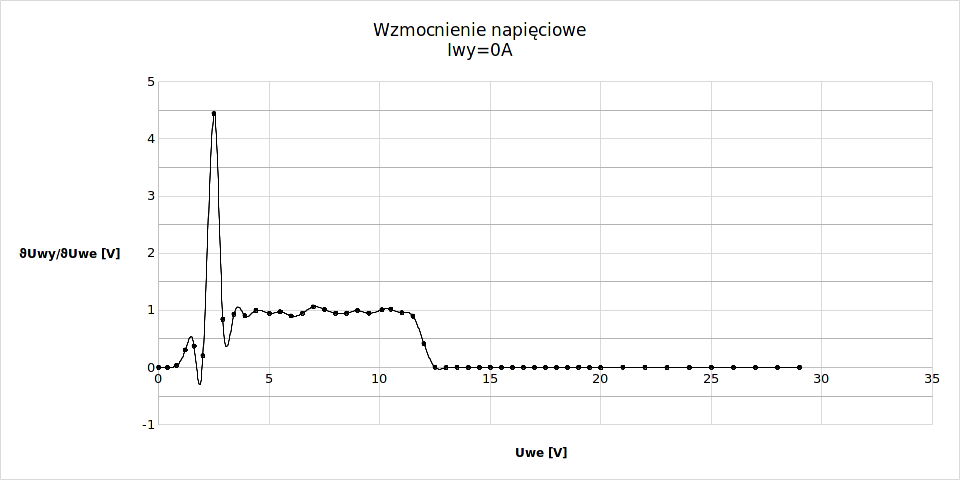
\includegraphics[width=1\textwidth]{wzmocnienie1}
  \caption{ $\frac{\partial U\textsubscript{wy}}{\partial U\textsubscript{we}}=f(U_{we})$ przy I\textsubscript{wy}=0A}
\end{figure}

\begin{figure}[h!]
  \center
  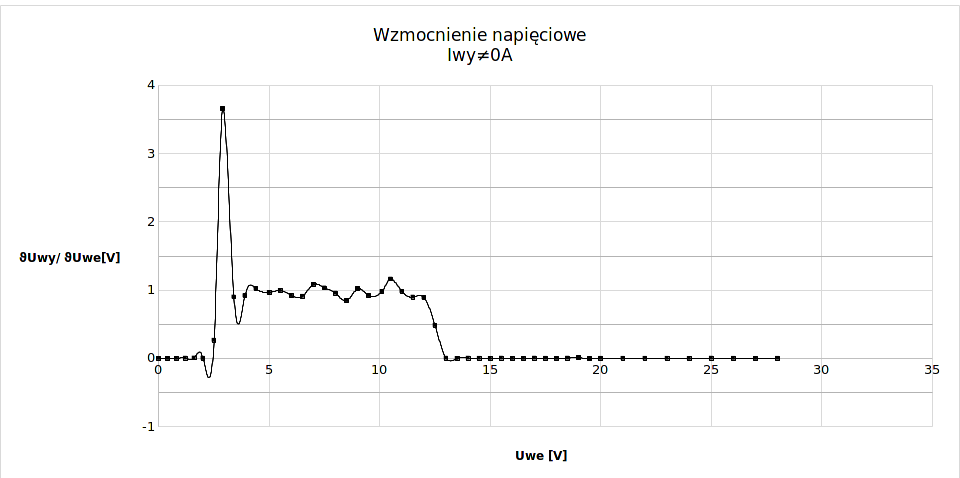
\includegraphics[width=1\textwidth]{wzmocnienie2}
  \caption{ $\frac{\partial U\textsubscript{wy}}{\partial U\textsubscript{we}}=f(U_{we})$ przy I\textsubscript{wy}\neq0A}
\end{figure} 

Współczynnik stabilizacji napięciowej w pewnym momencie bardzo gwałtownie się zmienia z uwagi na to, iż wcześniej prąd dostarczany do układu był
zbyt niski aby stabilizator zaczął pracować .Fragment przejściowy charakterystyk z rysunków 3 i 4 odpowiadaja fragmentom oscylującym w okół
jedynki na rysunkach 5 i 6. Oscylacje są prawdopodobnie spowodowane niedokładnością przyrządów pomiarowych.

\pagebreak
%%%%%%%%%%%%%%%%%%%%%%%%%%%%%%%%%%%%%%%%%%%%%%%%%%%%%%%%%%%%%%%%%%%%%%%%%%%%%%%%%%%%%%%%%%%%%%%%%%%%%%%%%%%%%%%%%%%%%%%%%%%%%%%%%%%%%%%%%%%%%%%%%%%%
\subsection{Charakterystyki zewnętrzne}
\begin{table}[h]
\centering 
\begin{tabular}{|r|r|r|}
\hline
\multicolumn{1}{|l|}{Iwy {[}A{]}} & \multicolumn{1}{l|}{\partial Uwy/ \partial Iwy[\frac{V}{A}]}&
\multicolumn{1}{l|}{\partial Uwy/ \partial Iwy[\frac{V}{A}]} \\ \hline
\multicolumn{3}{|c|}{Uwe=15V}                                                                              \\ \hline
0.72                              & 0.04                            & \multicolumn{1}{c|}{-}               \\ \hline
0.72                              & 3.81                            & -3775.80                             \\ \hline
0.72                              & 4.99                            & 317.49                               \\ \hline
0.72                              & 7.31                            & 4645.20                              \\ \hline
0.72                              & 10.88                           & -488.36                              \\ \hline
0.55                              & 10.96                           & -0.50                                \\ \hline
0.37                              & 10.97                           & -0.07                                \\ \hline
0.29                              & 10.98                           & -0.08                                \\ \hline
0.20                              & 10.99                           & -0.07                                \\ \hline
0.14                              & 10.99                           & -0.08                                \\ \hline
0.09                              & 10.99                           & -0.08                                \\ \hline
0.07                              & 11.00                           & -0.06                                \\ \hline
0.05                              & 11.00                           & 0.00                                 \\ \hline
\multicolumn{3}{|c|}{Uwe=30V}                                                                              \\ \hline
0.29                              & 0.01                            & \multicolumn{1}{c|}{-}               \\ \hline
0.40                              & 2.08                            & -18.73                               \\ \hline
0.47                              & 3.20                            & -15.96                               \\ \hline
0.71                              & 7.11                            & -16.27                               \\ \hline
0.71                              & 10.71                           & 4000.00                              \\ \hline
0.55                              & 10.96                           & 1.53                                 \\ \hline
0.37                              & 10.97                           & 0.08                                 \\ \hline
0.29                              & 10.98                           & 0.11                                 \\ \hline
0.20                              & 10.99                           & 0.08                                 \\ \hline
0.14                              & 10.99                           & 0.09                                 \\ \hline
0.09                              & 11.00                           & 0.10                                 \\ \hline
0.07                              & 11.00                           & 0.11                                 \\ \hline
0.05                              & 11.00                           & 0.04                                 \\ \hline
\end{tabular}
\end{table}
%%%%%%%%%%%%%%%%%%%%%%%%%%%%%%%%%%%%%%%%%%%%%%%%%%%%%%%%%%%%%%%%%%%%%%%%%%%%%%%%%%%%%%%%%%%%%%%%%%%%%%%%%%%%%%%%%%%%%%%%%%%%%%%%%%%%%%%%%%%%%%%%%%%%
\pagebreak

\begin{figure}[h]
  \center
  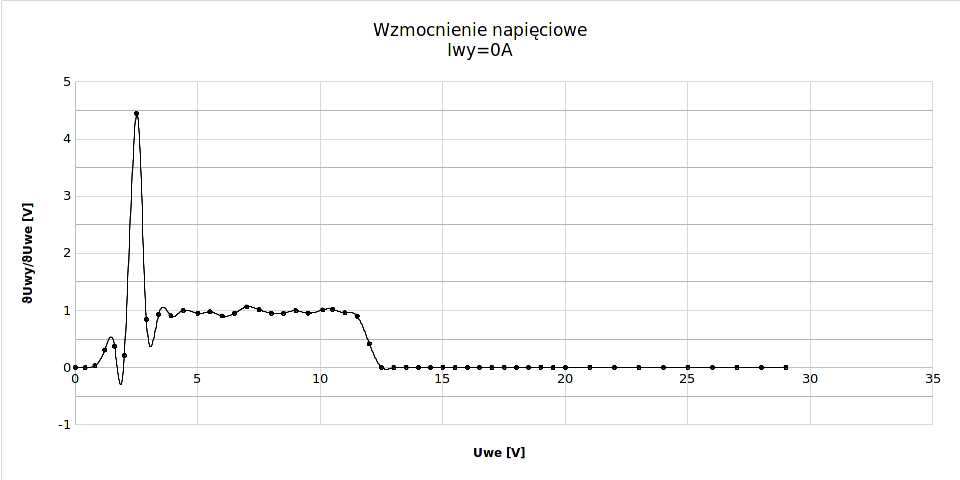
\includegraphics[width=0.9\textwidth]{charak-zew1}
  \caption{U\textsubscript{wy}=f(I\textsubscript{wy}) przu U\textsubscript{we}=15V}
\end{figure}

\begin{figure}[h]
  \center
  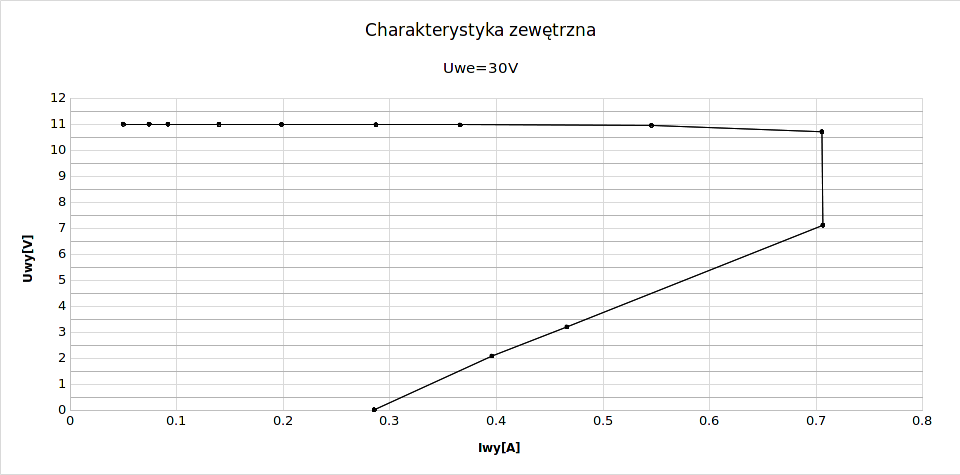
\includegraphics[width=0.9\textwidth]{charak-zew2}
  \caption{U\textsubscript{wy}=f(I\textsubscript{wy}) przu U\textsubscript{we}=30V}
\end{figure}

Analizując charakterystyki zewnętrzne stabilizatora zauważamy, że przy U\textsubscript{we}=15V układ nie przepuszcza prądu powyżej zadanych 0.70A.


\pagebreak
%%%%%%%%%%%%%%%%%%%%%%%%%%%%%%%%%%%%%%%%%%%%%%%%%%%%%%%%%%%%%%%%%%%%%%%%%%%%%%%%%%%%%%%%%%%%%%%%%%%%%%%%%%%%%%%%%%%%%%%%%%%%%%%%%%%%%%%%%%%%%%%%%%%%
\subsection{Impedancja wyjściowa}

\begin{figure}[h]
  \center
  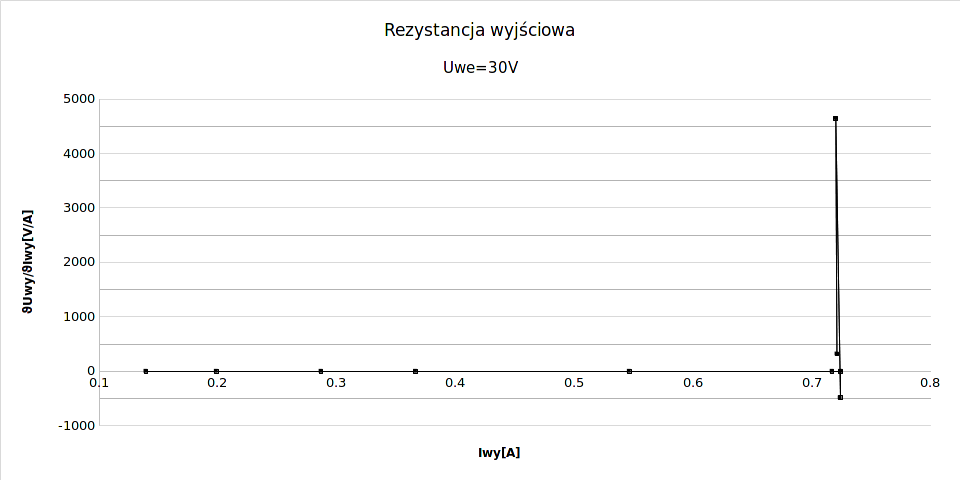
\includegraphics[width=0.9\textwidth]{rezystancja1}
  \caption{U\textsubscript{wy}=f(I\textsubscript{wy}) przu U\textsubscript{we}=15V}
\end{figure}

\begin{figure}[h]
  \center
  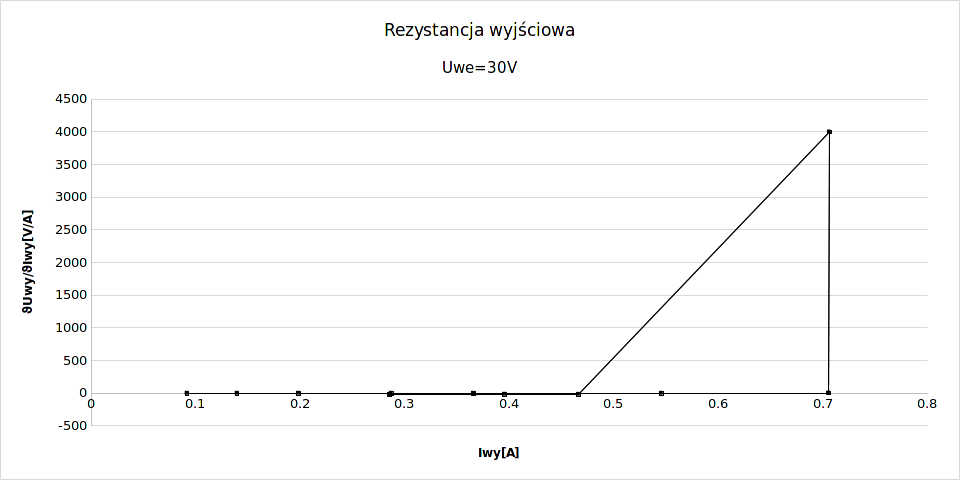
\includegraphics[width=0.9\textwidth]{rezystancja2}
  \caption{U\textsubscript{wy}=f(I\textsubscript{wy}) przu U\textsubscript{we}=30V}
\end{figure}

Do około 0.7 A układ utrzymuje stałą rezystancję wewnętrzną rzędu kilku omów/części dziesiętnych omów , po przekroczeniu tej wartości następuje
nagły wzrost rezystancji, który przeciwdziała przekroczeniu zadanego napięcia. Na rysunku nr.9  obserwujemy tzw. foldback
('odwijanie' charakterystyki) co jest zabezpieczeniem układu w wypadku dalszego wzrostu napięcia wejściowego.

\pagebreak
%%%%%%%%%%%%%%%%%%%%%%%%%%%%%%%%%%%%%%%%%%%%%%%%%%%%%%%%%%%%%%%%%%%%%%%%%%%%%%%%%%%%%%%%%%%%%%%%%%%%%%%%%%%%%%%%%%%%%%%%%%%%%%%%%%%%%%%%%%%%%%%%%%%%
\section {Wnioski}

\begin{enumerate}
  
\item Zgodnie z założeniami teoretycznymi układ utrzymuje na swoim wyjściu stałe napięcie równe 11V , w związku z niedokładnością użytych
  elementów maksymalny prąd wyjściowy różni się od założeń jednak nie jest to duża rozbieżność (około 0.70 A wobec założonych 0.66 A).
  
\item Minimalny spadek napięcia pomiędzy wyjściem a wejściem stabilizatora, potrzebny do właściwej stabilizacji napięcia wyjściowego (dropout) dla I\textsubscript{wy}=0 wynosi około 1.5V a dla I\textsubscript{wy}\neq0$ około 2V. Z czego wynika, iż wraz ze wzrostem
  obciążenia dropout również rośnie
  
\item W stabilizatorze kompensacyjnym udało nam się zaobserwować tzw.foldback który jest bardzo dobrym zabezpieczeniem układu w wypadku podawania
  na wejście zbyt dużych wartości napięć.

  
\end{enumerate}
\end{document}
